\documentclass{article}
\pdfpagewidth=8.5in
\pdfpageheight=11in
\usepackage{ijcai27}
\usepackage[T1]{fontenc}
\usepackage{times}
\usepackage{url}
\usepackage[hidelinks]{hyperref}
\usepackage[small]{caption}
\usepackage{graphicx}
\usepackage{amsmath,amssymb,booktabs}
\usepackage[switch]{lineno}
\linenumbers
\urlstyle{same}
% Preserve the official metadata block when building with XeTeX/Tectonic.
\ifdefined\pdfinfo\else
\def\pdfinfo#1{\special{pdf:docinfo << #1 >>}}
\fi
\pdfinfo{/TemplateVersion (IJCAI.2027.0)}
\title{When Forecasting Gains Do Not Establish Alpha:\\An Evidence Audit of Financial Machine Learning}
\author{Anonymous Authors\\Research draft: evidence and author approval pending}
% Claim/source bindings are recorded in evidence/claim_evidence.csv.
% This is a draft, not an assertion of a completed systematic replication study.
\begin{document}
\raggedbottom
\maketitle

\begin{abstract}
Financial prediction benchmarks can reward forecasting improvements without establishing investable, risk-adjusted gains. We audit a local research collection using a specified evaluation design: Chen--Zimmermann characteristics, exclusion of stocks below the lagged NYSE size twentieth percentile, value-weighted top-minus-bottom deciles, transaction-cost scenarios, and Fama--French five-factor plus momentum alpha with dependence-robust uncertainty. The collection contains a 437-paper catalogue, but its legacy evaluations do not establish compliance with this design. One completed compatible experiment identified in the audit transfers LiMT to historical US large-cap equities with 202 retained characteristics and three-seed score averaging. Across 2,260 trading days in 2017--2025, its annual alpha is 5.31\% before costs (95\% HAC interval $[-2.54,13.16]$\%, $p=0.185$) and $-1.27$\% under a 10-basis-point all-trade cost scenario ($[-9.11,6.56]$\%, $p=0.750$). Neither establishes positive alpha. These findings do not prove zero profitability or inferiority to a dummy baseline. We distinguish profitability, incremental performance, and evidence of economically negligible effects, and propose publication requirements that align financial ML claims with the statistical and economic quantities actually tested.
\end{abstract}

\section{Introduction}
% C01: protocol and primary results; C02: scope of collection.
A return-prediction model may improve a benchmark score while leaving an investor with an uncertain economic benefit. The relevant claim is not exhausted by a positive return estimate: trading rules, capitalization weights, factor exposures, implementation costs, and sampling uncertainty determine what that estimate establishes. Financial ML publications that claim profitable trading should therefore identify the investment proposition being tested and report evidence for that proposition.

We ask what the available evidence establishes when a financial ML model is evaluated under an explicit investment protocol. A completed LiMT transfer does not establish significant positive alpha under the specified design. The broader collection, however, is not a set of completed comparable experiments, and other saved designs contain positive gross-return evidence. This setting exposes two evaluation problems: catalogue size can overstate empirical coverage, and a non-significant return estimate can be misread as proof of baseline inferiority. An evidence audit must address both before drawing conclusions about an architecture or the field.

Our evaluation design, supplied before this manuscript audit, combines individual-stock Chen--Zimmermann (CZ) characteristics, a lagged NYSE twentieth-percentile microcap screen, value-weighted D10$-$D1 portfolios, gross and after-cost returns, and FF5 plus momentum regressions. These components have precedents in empirical asset pricing, but their exact combination is a study specification rather than a universal definition of financial usefulness. In particular, changing a model's input family or market is a transfer experiment, not necessarily a replication of its published claim.

The contribution is threefold. First, we separate catalogue coverage from completed return evidence, preventing missing experiments from being counted as failures. Second, we independently reconstruct the reported uncertainty of a completed CZ202 LiMT experiment from saved return ledgers and factor observations. Third, we give an operational reporting standard for profitability and baseline comparisons. We do not introduce a new forecasting architecture or claim a field-wide impossibility result.

\section{Related Evidence and Scope}
% C03--C07: targeted source assessment; not a systematic review.
\paragraph{Investability and replication.}
Anomaly evidence depends on the object being reproduced. \cite{hou2017} emphasize microcap treatment and value weighting in an extensive replication exercise. \cite{chen2022} instead report strong reproduction of predictors with clear original evidence and distinguish those predictors from insignificant or modified characteristics. Their findings caution against treating a changed portfolio specification as a faithful test of every original finding. We use CZ as a standardized stock-characteristic source, not as proof that all its constituent predictors either work or fail under our design.

Trading costs also change the question. \cite{novymarx2016} study cost mitigation and show why turnover and entry/retention rules matter. \cite{avramov2023} report that restrictions involving microcaps, distress, volatility states, and trading costs attenuate ML-based performance. These results motivate testing implementation assumptions explicitly. They do not imply that every ML strategy has negative expected returns.

\paragraph{Evidence against a universal negative claim.}
\cite{gu2020} report economic gains from trees and neural networks; their published analysis includes value-weighted decile portfolios, factor-adjusted performance, and a microcap-exclusion sensitivity. These dimensions are consequently not absent from finance ML as a whole. An archived working-paper version of \cite{azevedo} also reports positive after-cost ML strategy evidence, while considering publication timing and modern trading conditions. We reviewed the archived version available through the American Finance Association; we do not treat its estimates as a replication under the present protocol. The appropriate question is which methods and conditions survive a specified test, rather than whether ML can ever be useful in finance.

\paragraph{Statistical selection.}
\cite{harvey2016} explain why extensive factor searches require stronger evidence than an isolated nominal significance test. \cite{white2000} explicitly formulates data-snooping-adjusted comparison with a benchmark. The present audit retains the experiment's within-family adjustment, but does not claim to recover the full historical search over models, datasets, or research specifications. Likewise, repeating training seeds on the same return dates does not create new independent market histories.

\paragraph{Review boundary.}
The literature extension is a targeted narrative review, searched on 10 November 2026 using public scholarly and author/publisher sources. It covers competing profitability findings, replication design, costs, and inference. It is not an exhaustive systematic review, and its references are not additional completed experiments. The local 437-record workbook is a supplied convenience collection, not a probability sample of all ML publications. It also includes financial tasks without an investment-return estimand.

\section{What the Protocol Tests}
% C08: definition derived from protocol.txt and experiment specification.
\subsection{Investment Universe and Portfolio}
At a signal date in month $m$, let $M_{i,m-1}$ be stock $i$'s observed capitalization at the previous calendar month end. Let $q_{.20,m-1}^{\mathrm{NYSE}}$ be the twentieth percentile among eligible NYSE common stocks at that time. The microcap condition is
\begin{equation}
M_{i,m-1}\geq q_{.20,m-1}^{\mathrm{NYSE}},
\end{equation}
with positive observed capitalization required. Unknown capitalization is excluded separately and counted. Membership, characteristic availability, and any additional universe restrictions must also be documented. This screen does not authorize selecting stocks on their future returns or survival.

Rank eligible stocks by a model score whose direction is fixed before evaluating returns. Let $L_t$ and $S_t$ be the top and bottom deciles. Ideal capitalization weights are
\begin{equation}
w^*_{i,t}=\frac{M_{i,m-1}\mathbf{1}(i\in L_t)}{\sum_{j\in L_t}M_{j,m-1}}
-\frac{M_{i,m-1}\mathbf{1}(i\in S_t)}{\sum_{j\in S_t}M_{j,m-1}}.
\end{equation}
This is a conventional $+100\%/-100\%$ spread with 200\% gross exposure. Its scale must be stated: a $+50\%/-50\%$ portfolio has half the arithmetic return and alpha under exact linear scaling, while its mean-test statistic is unchanged. Compound wealth and cost-dependent execution require the actual ledger. Dollar neutrality alone does not imply zero market beta or neutrality to other factors.

For executed weights $w_{i,t}$, asset total returns $r_{i,t}$, and return-unit costs $c_t$, define
\begin{equation}
R_t^{\mathrm{gross}}=\sum_i w_{i,t}r_{i,t},\qquad
R_t^{\mathrm{net}}=R_t^{\mathrm{gross}}-c_t.
\end{equation}
Portfolio targets and actual holdings can differ when positions cannot be traded. Return accounting must retain the resulting exposure, turnover, dividends, terminal payoffs, and missing-payoff diagnostics. A target-decile return table cannot substitute for an executed-holdings ledger.

\subsection{Risk Adjustment and Uncertainty}
The primary regression is
\begin{equation}
R_t=\alpha+\boldsymbol\beta^{\top}\mathbf f_t+\varepsilon_t,
\label{eq:alpha}
\end{equation}
where $\mathbf f_t$ contains market excess return, SMB, HML, RMW, CMA, and the French momentum series used as UMD. Factor definitions follow the official Data Library \cite{french}. The zero-investment spread is regressed directly on these factors; the risk-free rate is not subtracted again. We estimate gross and after-cost intercepts separately. Alpha is conditional on this factor model, not a model-free measure of skill or an executable hedge fitted in advance.

The completed daily experiment uses Bartlett HAC covariance with 20 lags, a finite-sample covariance correction, and two-sided $t$-reference intervals. Annual alpha is $252\widehat\alpha$; it is not CAGR. Dependence-robust covariance follows the principle of \cite{newey1987}. Results at 5 and 60 lags are retained as sensitivities. An individual 95\% interval is not a simultaneous interval for a searched family of strategies.

Positive-alpha evidence requires a positive estimate with the lower confidence bound above zero. A family-level assertion also requires the declared multiplicity procedure. This is an evidential requirement for an alpha claim, not a proposal to publish only significant results. Inconclusive results, negative estimates, and failed replications remain scientifically relevant when their design and precision are informative.

\section{Evidence Audit and Completed Experiment}
% C09--C13: coverage snapshot and local protocol.
\subsection{Coverage Is Not a Failure Rate}
The supplied catalogue contains 437 records. Its programme snapshot, timestamped 9 November 2026, describes an ongoing workflow. Its primary legacy return extension uses zero implementation costs and $+50\%/-50\%$ holdings; it does not certify CZ202 inputs, capitalization weighting, the required size screen, or FF5+UMD alpha. Table~\ref{tab:coverage} preserves that extension's recorded categories. They cannot be pooled into a protocol-compliant success rate.

\begin{table}[t]
\centering
\begin{tabular}{lr}
\toprule
Legacy return-extension category & Records\\
\midrule
Pending & 273\\
Blocked & 52\\
Not applicable & 110\\
Completed, positive but inconclusive & 2\\
\midrule
Total catalogue & 437\\
\bottomrule
\end{tabular}
\caption{Recorded paper-level categories in the legacy programme snapshot. These are metadata under a different protocol, not outcomes of 437 completed CZ202 experiments. Workflow completion and return-extension completion are separate fields.}
\label{tab:coverage}
\end{table}

One completed compatible experiment identified in this audit is the LiMT CZ202 US transfer. A separate all-nonmicrocap CS-GAT protocol has a prepared input panel but no completed return-inference artifact in the inspected snapshot. It contributes no result here. Generic architectures, credit-risk classifiers, financial question-answering systems, and unavailable or unfinished runs are not counted as unprofitable strategies. For example, applying ArbNN \cite{yan2026} to a newly constructed stock-ranking task does not directly test its original credit-risk claims.

\subsection{LiMT Transfer Design}
LiMT combines cross-stock and temporal modeling with liquidity-related auxiliary objectives \cite{yang2026}. The completed local transfer uses a changing historical US largest-500 common-stock universe, followed by the explicit lagged NYSE size screen and CZ-record availability requirements. It therefore covers a large-cap subset of the eligible stock universe, not all nonmicrocap CRSP stocks.

The official October 2026 CZ stock-level release supplies 209 available characteristics. Seven training-constant columns are dropped, leaving 202. Price, Size, and STreversal are absent from the public file and are not reconstructed. Within each source month, observed values are ranked over the available nonmicrocap common-stock population, average ties are mapped to $[-1,1]$, and missing values are mapped to neutral zero. These are stock-level predictors, not returns on factor portfolios. Each daily input uses only the preceding calendar month's characteristics; there is no future fill or stale carry across missing source months. The source release documents revisions and unequal end dates for some signals \cite{czdata}.

Training covers 2008--2014; validation covers 2015--2016; test forecasts cover 2017--2025. The implementation checks that label realizations do not cross training/validation boundaries. It uses a 21-session lookback, the full local model configuration, three seeds, and validation daily return IC for checkpoint selection. The three prediction scores are averaged before ranking. Training labels retain daily price-return and liquidity-related auxiliary targets, while portfolio payoffs use CRSP total returns. Monthly characteristics repeated in a daily forecasting architecture are a substantive input change from the original task.

The saved protocol fixes signal at session $t$, assumed execution at $t+1$ close, and total-return payoff at $t+2$. Capitalization weights use the previous month end. The execution projection preserves frozen positions and imposes dollar neutrality. No observed stock-loan locates or actual closing fills are supplied. The after-cost scenario charges 10 basis points per dollar bought or sold, including establishment and terminal liquidation; it omits borrow fees, financing, market impact, and collateral yield. We therefore call it an after-trading-cost scenario, not a fully implemented net-investor return.

The experiment is retrospective. Its source, code, and input hashes were saved before this training run, but earlier experiments had already been examined. The specification is not a preregistered independent confirmation. Current-vintage CRSP and CZ data do not establish historical as-published availability.

\subsection{Independent Recalculation}
The manuscript audit reads existing artifacts without retraining or selecting a new model. It checks completion of all three seeds, frozen input hashes, saved output hashes, feature count, timestamp ordering, ledger identities, cost arithmetic, date uniqueness, factor coverage, and net exposure. It recomputes all 36 saved intercept tests using a separate NumPy implementation of the HAC sandwich covariance and reconstructs the Holm adjustment. The family comprises two weights, two costs, three windows, and three intercept specifications. This adjustment does not cover all earlier research decisions.

We additionally compute circular paired block-bootstrap percentile intervals for the full-period value-weighted alpha, resampling returns and factors together in blocks of 20 or 60 sessions, with 2,000 draws per case. These are newly added, post hoc robustness diagnostics. They do not turn an already inspected sample into confirmatory evidence. Source-holdings replay was recorded by the original experiment; our recalculation verifies the saved summaries and ledger arithmetic rather than claiming a new end-to-end raw-data reconstruction.

\section{Results}
% C14--C19: generated independent_hac.csv and primary_results.csv.
\subsection{Positive Returns Do Not Establish Positive Alpha}
The full-period ledger has 2,260 daily observations from 5 January 2017 to 31 December 2025. Value-weighted D10$-$D1 earns a positive annual arithmetic mean of 9.35\% gross and 2.77\% under the 10 bp cost scenario. Its CAGRs are 7.84\% and 0.97\%, respectively. The corresponding mean-return tests are inconclusive ($p=0.091$ and $p=0.617$). It would be incorrect to describe these realized returns as uniformly negative.

Table~\ref{tab:primary} reports the primary risk-adjusted quantities. Gross FF5+UMD alpha is 5.31\% per year, with a 95\% HAC interval spanning $-2.54\%$ to 13.16\%. After the stated trading costs, the estimate is $-1.27\%$, with an interval spanning $-9.11\%$ to 6.56\%. Neither result establishes positive alpha even before multiple-testing adjustment. Holm-adjusted $p$-values are both 1.000. Figure~\ref{fig:alpha} shows the uncertainty directly.

\begin{table}[t]
\centering
\begin{tabular}{lrr}
\toprule
Quantity & Gross & 10 bp\\
\midrule
Annual arithmetic mean (\%) & 9.35 & 2.77\\
Annual FF5+UMD alpha (\%) & 5.31 & $-1.27$\\
95\% HAC lower bound (\%) & $-2.54$ & $-9.11$\\
95\% HAC upper bound (\%) & 13.16 & 6.56\\
HAC $t$-statistic, alpha & 1.326 & $-0.318$\\
Two-sided $p$, alpha & 0.185 & 0.750\\
Holm36 $p$, alpha & 1.000 & 1.000\\
\bottomrule
\end{tabular}
\caption{LiMT CZ202 US transfer, capitalization-weighted D10$-$D1, $+100\%/-100\%$ target exposures, 2,260 days in 2017--2025. Alpha and mean are annual arithmetic quantities; intervals are individual HAC(20) intervals. Costs omit borrowing, financing, impact, and collateral yield.}
\label{tab:primary}
\end{table}

\begin{figure}[t]
\centering
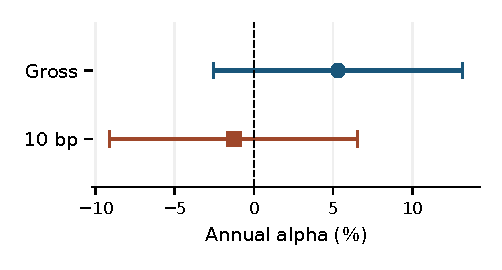
\includegraphics[width=\columnwidth]{figures/alpha_intervals.pdf}
\caption{Annual value-weighted FF5+UMD alpha with individual 95\% HAC(20) intervals. Both intervals contain zero and economically material positive and negative values. Shapes distinguish cost scenarios without relying on color.}
\label{fig:alpha}
\end{figure}

Supplementary raw-share-volume weighting also fails to establish positive full-period alpha: estimates are 9.13\% gross ($p=0.216$) and $-8.81\%$ after costs ($p=0.233$). Raw share volume depends on share units and is not interchangeable with capitalization or dollar volume. These rows are retained to disclose the evaluated variants, not to replace the primary weighting after observing results.

\subsection{Robustness and Precision}
The newly computed 20-session bootstrap alpha intervals are $[-2.24,12.96]$\% gross and $[-9.73,6.02]$\% after costs. With 60-session blocks they are $[-2.62,12.86]$\% and $[-9.40,6.21]$\%. Their qualitative interpretation agrees with the HAC intervals. Neither bootstrap design addresses unseen implementation costs or an unrecorded research search.

The value-weighted ledger contains two missing held-payoff records. The saved adverse diagnostic assigns an underlying return of $-100\%$ for a missing long payoff and $+100\%$ for a missing short payoff, keeping the selections fixed. Gross annual alpha becomes 5.17\% ($p=0.196$). This is a finite sensitivity, not a worst-case bound on short losses. In the universe audit, only eight of 1,131,000 original test stock-days are removed for falling below the lagged size threshold. The primary universe was already concentrated in large firms, so this experiment does not identify the isolated causal effect of eliminating microcaps.

The intervals remain wide. In particular, the after-cost alpha upper bound of 6.56\% prevents us from excluding economically meaningful positive performance. A significance threshold alone cannot turn such uncertainty into evidence of economic irrelevance. Both negative and positive effect sizes compatible with the sample should remain visible.

\subsection{Other Saved Designs Prevent a Universal Claim}
The earlier US LiMT experiment with Alpha158 inputs and equal-dollar ranking portfolios reports a significant positive gross annual mean of 12.04\% ($p=0.000218$; within-family Holm $p=0.00457$). Its 5 bp buy-side-only cost sensitivity is not significant. The local zero-cost audit also records significant gross means in two Chinese LiMT universes. These are different estimands and designs: they are neither protocol-compliant successes nor failures of the CZ202 test. They nevertheless rule out describing the entire directory as containing no positive gross-return evidence. Because inputs, weights, and cost conventions change together, the contrast is not an ablation identifying which change explains the difference.

\section{What Would Establish Baseline Inferiority?}
% C20: mathematical interpretation, not an empirical finding.
\subsection{Three Distinct Claims}
\textbf{Profitability.} A positive-alpha assertion concerns Equation~\ref{eq:alpha}. Positive realized mean returns can coexist with non-significant or negative alpha, and positive alpha can coexist with unmodeled implementation costs. Authors must state which quantity supports their economic claim.

\textbf{Incremental value.} To compare model $A$ with a baseline $B$, evaluate a paired difference on common dates under matched eligibility, exposure, and cost rules:
\begin{equation}
\Delta_t=R^A_t-R^B_t.
\end{equation}
Estimate its mean or factor-adjusted intercept with dependence-robust uncertainty. If the entire interval is below zero, the comparison supports inferiority for that estimand. A non-significant test of $A$ against zero does not supply this result. Nor does the difference between two separate significance labels test the difference between models.

\textbf{Economic negligibility.} Before evaluating outcomes, choose a practically meaningful annual margin $\delta$. Equivalence requires an appropriate equivalence procedure, such as two one-sided tests with the corresponding interval wholly inside $(-\delta,\delta)$. A non-inferiority claim uses its own one-sided margin and direction. Neither property follows from an ordinary $p>0.05$. The current intervals are too broad to support a general assertion of negligible alpha.

\subsection{The Dummy Baseline Must Be Defined}
A constant return forecast gives all stocks equal scores. Without a tie rule, a D10$-$D1 portfolio is undefined and may spuriously trade an identifier ordering. A coherent no-information control can assign identical fractional membership to both extreme deciles so the long and short positions cancel; it then produces no trades and a zero spread. This convention is an analytical definition, not a newly executed experiment in this paper. The no-trade control has no meaningful Sharpe ratio because its volatility is zero. Its zero alpha does not make a noisy model statistically inferior.

A no-trade control is also insufficient as the only comparator. A serious architecture-value claim should include a matched linear or ridge model, a competitive tree model, and simple lagged signals, as appropriate to the task. A positive ML alpha alone does not prove improvement over them. No matched CZ202 baseline ledger is supplied by the completed experiment, so its incremental value remains untested here. A low forecast-error baseline, a no-trade portfolio, and an investable long-only market portfolio answer different questions and should not be conflated.

\section{A Publication Standard for Return Claims}
% C21: proposed requirements, not established venue rules.
We propose the following requirements for papers that claim profitable asset-return forecasting or superior trading performance. These are recommendations, not existing IJCAI requirements.

\paragraph{1. Declare the economic estimand.}
Specify the market, eligible universe, source vintages, information lags, holding horizon, score direction, portfolio weights, gross/net exposure, tie rule, and benchmark. Label faithful replications, method transfers, and exploratory adaptations separately. Explain which scientific claim the test can refute.

\paragraph{2. Make the backtest auditable.}
Retain predictions and an ordered holdings/cash/NAV ledger, corporate-action treatment, missing-payoff counts and weights, turnover, initial trades, liquidation, and actual departures from target positions. Report the observed size-screen removals. A positive Sharpe ratio or a prediction table alone is insufficient evidence of executable trading.

\paragraph{3. Report uncertainty on both returns and alpha.}
Give estimates, dependence-robust standard errors, signed test statistics, confidence intervals, and $p$-values for gross and stated after-cost returns. Report factor exposures and explain factor choice. Show economically meaningful units and separate annual arithmetic quantities from compounded growth. Test an economically motivated margin when asserting that an effect is negligible.

\paragraph{4. Test paired baseline improvements.}
Use common return dates and comparable execution assumptions. Provide a no-information control and credible simple predictive baselines. Estimate uncertainty for the paired increment rather than inferring superiority from separate point estimates or separate significance decisions. Disclose differences in model-selection budgets and missing-outcome coverage.

\paragraph{5. Account for selection and implementation.}
Freeze checkpoints and score direction using training/validation information. Disclose all tested seeds, horizons, universes, costs, windows, and variants, identifying the multiplicity family and unresolved prior search. Preserve nominal and adjusted evidence together. Include turnover-linked cost sensitivities and distinguish assumed costs from observed fills, borrowing availability, financing, and impact. A zero-cost result can test signal content without establishing deployable profits.

\paragraph{6. Publish informative null findings.}
Neither an access failure nor an unfinished experiment is a null return result. Conversely, a transparent negative or inconclusive finding can illuminate precision, domain transfer, or a model failure mode. Statistical significance should discipline claims rather than become a filter that suppresses null evidence or rewards ever larger searches. Financial NLP, credit risk, fraud detection, and risk forecasting should be evaluated against their own declared decision objectives when profitable stock selection is not the claimed contribution.

\section{Limitations and Conclusion}
The principal limitation is breadth: this audit identifies one completed compatible model family, not a completed protocol-compliant census. The large-cap universe, retrospective current-vintage inputs, daily use of monthly predictors, fixed training interval, and idealized execution restrict generalization. The original LiMT paper studies different benchmarks and inputs; this transfer cannot establish that its original results are incorrect. Our statistical recalculation is independent of the saved inference implementation, but relies on the same historical market observations. The targeted literature review does not estimate a field-wide replication rate.

The defensible empirical statement is that the completed LiMT CZ202 transfer does not establish positive FF5+momentum alpha, either gross or under the stated cost scenario. Its uncertainty does not establish zero profitability, economic negligibility, or inferiority to a dummy baseline. Future finance ML publications making return claims should connect them to auditable portfolios, matched baseline increments, explicit implementation assumptions, and selection-aware statistical uncertainty. Those requirements permit strong claims when supported and informative negative evidence when they are not.

\section*{Ethical Considerations}
This manuscript concerns evaluation methodology and retrospective financial research. No strategy was deployed by this manuscript audit. CRSP and other licensed underlying data require their applicable access permissions; a local file's existence does not establish redistribution rights. The proposed artifact release should contain permitted code, aggregate results, and data-reconstruction instructions rather than restricted source data. Availability and release permissions remain to be finalized by the accountable authors.

\clearpage
\bibliographystyle{named}
\bibliography{references}
\end{document}
